\documentclass[12pt,a4paper]{scrartcl}
\usepackage[utf8]{inputenc}
\usepackage[english,russian]{babel}
\usepackage{indentfirst}
\usepackage{misccorr}
\usepackage{graphicx}
\usepackage{amsmath}
\usepackage{multirow}
\usepackage{pgfplots}
\usepackage{parskip}
\usepackage[top=1cm, bottom=1cm, left=1cm, right=1cm]{geometry}
\pgfplotsset{compat=1.9}

\begin{document}
	\graphicspath{{py/}}
	
	\newcommand{\ms}{\mathstrut}
	\newcommand{\msp}{\hspace{0.5cm}}
	\newcommand{\al}{\alpha}
	\newcommand{\dg}{^\circ}
	\newcommand{\dif}{\mathrm{d}}
	\newcommand{\qd}[2]{^{\frac{#1}{#2}}}
	\newcommand{\qdm}[2]{^{-\frac{#1}{#2}}}
	\newcommand{\lm}[2]{\underset{#1 \rightarrow #2}{\lim}}
	\newcommand{\sfrac}[2]{\dfrac{\strut #1}{\strut #2}}
	\newcommand{\equal}[1]{\overset{(#1)}{=}}
	\newcommand{\linevdots}{\ \raisebox{-.08\height}{\vdots}\ }
	\newcommand{\linecvdots}{\ \raisebox{-.08\height}{\vdots}\hspace{-0.13cm}\raisebox{.15\height}{\cancel{\phantom{a}}\hspace{0.06cm}}}
	\newcommand{\combox}[1]{\ms \msp \msp \begin{minipage}{0.95\linewidth}
			#1
	\end{minipage}}
	
	\newtheorem{pr}{Задача}
	\newtheorem{ex}{Пример}
	\newtheorem{dfn}{Def}
	\newtheorem{theorem}{Th}
	
	\newenvironment{slv}{\ms \msp \textit{Решение:}}{}
	\newenvironment{proof}{\ms \msp \textit{Доказательство: }}{\hfill $\square$}
	
	\begin{titlepage}
		
		\vspace*{\fill}
		
		\begin{center}
			
\includegraphics[scale=0.8]{MIPT.png}
			\\[0.7cm]\Huge Московский Физико-Технический Институт\\(национальный исследовательский университет)
			\\[2cm]\LARGE Отчет по эксперименту
			\\[0.5cm]\noindent\rule{\textwidth}{1pt}
			\\\Huge\textbf{Определение $C_p /C_v$ по скорости звука в газе}
			\\[-0.5cm]\noindent\rule{\textwidth}{1pt}
		\end{center}
		
		\begin{flushleft}
			\textit{Работа №2.1.3; дата: 22.04.22}\hfill\textit{Семестр: 2}
		\end{flushleft}
		
		\vspace*{\fill}
		
		\begin{flushleft}
			Выполнил: \hspace{\fill} Группа:
			\\Кошелев Александр \hspace{\fill} Б05-105
		\end{flushleft}
	\end{titlepage}
	
	%Страница 2
	
	\begin{flushleft}
		\footnotesize{Определение $C_p /C_v$ по скорости звука в газе} \hspace{\fill} \footnotesize{2}
		\\[-0.3cm]\noindent\rule{\textwidth}{0.3pt}
	\end{flushleft}
	
	\section{Аннотация}
	
	\textbf{Цель работы: }
	
	\begin{enumerate}
		\item Измерение частоты колебаний и длины волны при
		резонансе звуковых колебаний в газе, заполняющем трубу;
		\item Определение показателя адиабаты с помощью уравнения состояния идеального газа.
	\end{enumerate}
	
	\textbf{Схема установки:}
	\begin{center}
		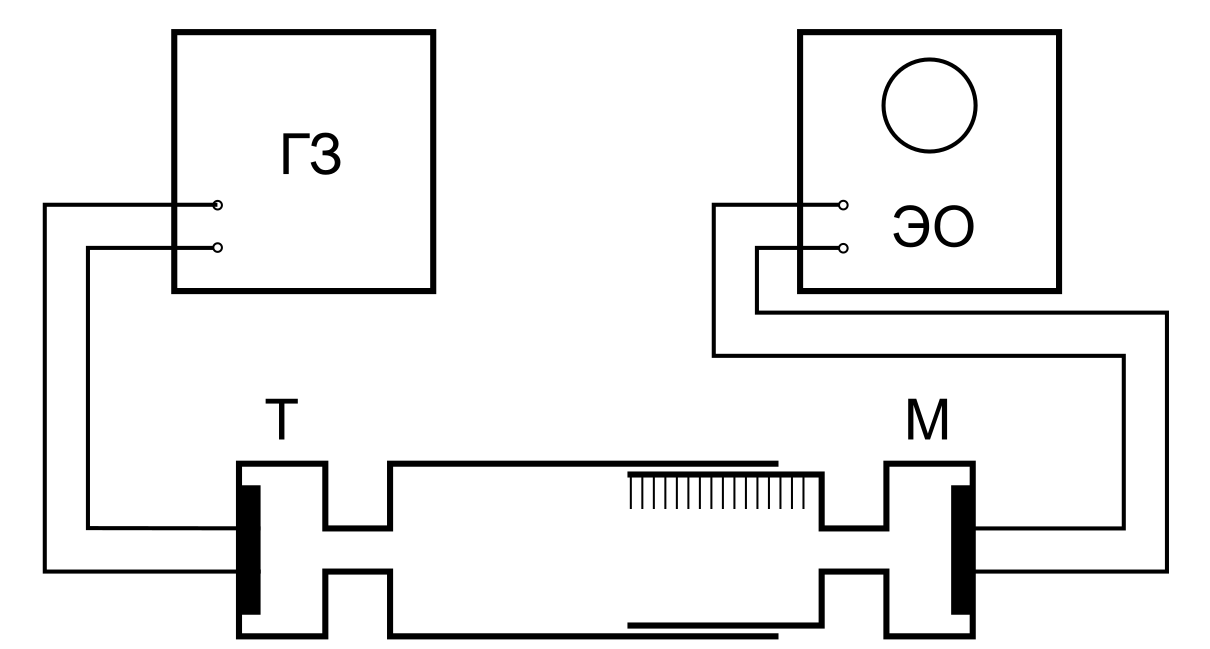
\includegraphics[scale=0.25]{PIC_1}
		\\\textbf{Рис. 1:} Схема установки
	\end{center}
		
	Установка содержит теплоизолированную трубу постоянной длины. Воздух в трубе нагревается водой из термостата. Температура газа принимается равной температуре омывающей трубу воды. На этой установке измеряется зависимость скорости звука от температуры.	
		
	\textbf{В работе используются:}
	
	Звуковой генератор ГЗ; электронный осциллограф ЭО; микрофон; телефон; раздвижная труба; теплоизолированная труба, обогреваемая водой из термостата; баллон со сжатым углекислым газом; газгольдер.
	
	\section{Теоретические сведения}
	Скорость распространения звуковой волны в газах зависит от показателя адиабаты $\gamma$. На измерении скорости звука основан один из наиболее точных методов определения показателя адиабаты. Скорость звука в газах определяется формулой:
	
	\begin{equation}
		c = \sqrt{\gamma \sfrac{RT}{\mu}} \implies \gamma = \sfrac{\mu}{RT}c^2
	\end{equation}

	Таким образом, для определения показателя адиабаты достаточно измерить температуру газа и скорость распространения звука (молярная масса газа предполагается известной).
	
	
	Звуковая волна, распространяющаяся вдоль трубы, испытывает многократные отражения от торцов. Звуковые колебания в трубе являются наложением всех отраженных волн и, вообще говоря, очень сложны. Картина упрощается, если длина трубы $L$ равна целому числу полуволн, то есть когда
	
	\begin{equation}
		L = \sfrac{n\lambda}{2}
	\end{equation}
	
	\newpage 
	
	%Страница 3
	
	\begin{flushleft}
		\footnotesize{Определение $C_p /C_v$ по скорости звука в газе} \hspace{\fill} \footnotesize{3}
		\\[-0.3cm]\noindent\rule{\textwidth}{0.3pt}
	\end{flushleft}
	
	Если условие (2) выполнено, то волна, отраженная от торца трубы, вернувшаяся к ее началу и вновь отраженная, совпадает по фазе с падающей. Совпадающие по фазе волны усиливают друг друга. Амплитуда звуковых колебаний при этом резко возрастает — наступает резонанс.
	
	При звуковых колебаниях слои газа, прилегающие к торцам трубы, не испытывают смещения (узел смещения). Узлы смещения повторяются по всей длине трубы через $\lambda/2$. Между узлами находятся максимумы смещения (пучности).
	
	Скорость звука c связана с его частотой $f$ и длиной волны $\lambda$ соотношением
	
	\begin{equation}
		c = \lambda f
	\end{equation}
	
	Подбор условий, при которых возникает резонанс, можно производить двояко:
	
	\begin{enumerate}
		\item При неизменной частоте $f$ звукового генератора (а следовательно, и неизменной длине звуковой волны $\lambda$) можно изменять длину трубы $L$. Для этого применяется раздвижная труба. Длина аздвижной трубы постепенно увеличивается, и наблюдается ряд последовательных резонансов. Возникновение резонанса легко наблюдать на осциллографе по резкому увеличению амплитуды колебаний. Для последовательных резонансов имеем
		
		$$L_n = n\sfrac{\lambda}{2},\ \ \ \ \ L_{n + 1} = (n + 1)\sfrac{\lambda}{2}, \ \ \ \ \ \ldots, \ \ \ \ \ L_{n + k} = (n + k)\sfrac{\lambda}{2}, $$
		
		т. е. $\lambda/2$ равно угловому коэффициенту графика, изображающего зависимость длины трубы $L$ от номера резонанса $k$. Скорость звука находится по формуле (3).
		
		\item При постоянной длине трубы можно изменять частоту звуковых колебаний. В этом случае следует плавно изменять частоту $f$ звукового генератора, а следовательно, и длину звуковой волны $\lambda$. Для последовательных резонансов получим
		
		$$L = \sfrac{\lambda_1}{2}n = \sfrac{\lambda_2}{2}(n + 1) = \ldots = \sfrac{\lambda_k}{2}(n + k)$$
	\end{enumerate}
	
	\section{Проведение эксперимента}
	\paragraph{Опыт с переменной длиной трубы для воздуха} \hfill
	
	Будем записывать величину вылета трубы для каждого из положений резонанса в таблице для нескольких разных частот звукового генератора.
	
	\begin{center}
		\begin{tabular}{|c|c|c|c|c|c|}
			\hline
			$f$, Гц & $2700 \pm 1$ &  $2998 \pm 1$ & $3502 \pm 1$ & $4042 \pm 1$ & $4476 \pm 1$
			\\\hline
			$i$, номер & \multicolumn{5}{|c|}{$((l - l_0) \pm 1)$, мм}
			\\\hline
			0 & 0 & 0 & 0 & 0 & 0
			\\\hline
			1 & 63 & 58 & 50 & 43 & 38
			\\\hline
			2 & 127 & 115 & 99 & 86 & 76
			\\\hline
			3 & 192 & 173 & 149 & 128 & 115
			\\\hline
			4 &     &     & 199 & 171 & 153
			\\\hline
			5 &     &     &     &     & 192
			\\\hline
		\end{tabular}
		\\\textbf{Табл. 1:} Первый опыт
	\end{center}
	
	\newpage 
	
	%Страница 4
	
	\begin{flushleft}
		\footnotesize{Определение $C_p /C_v$ по скорости звука в газе} \hspace{\fill} \footnotesize{4}
		\\[-0.3cm]\noindent\rule{\textwidth}{0.3pt}
	\end{flushleft}
	
	\begin{center}
		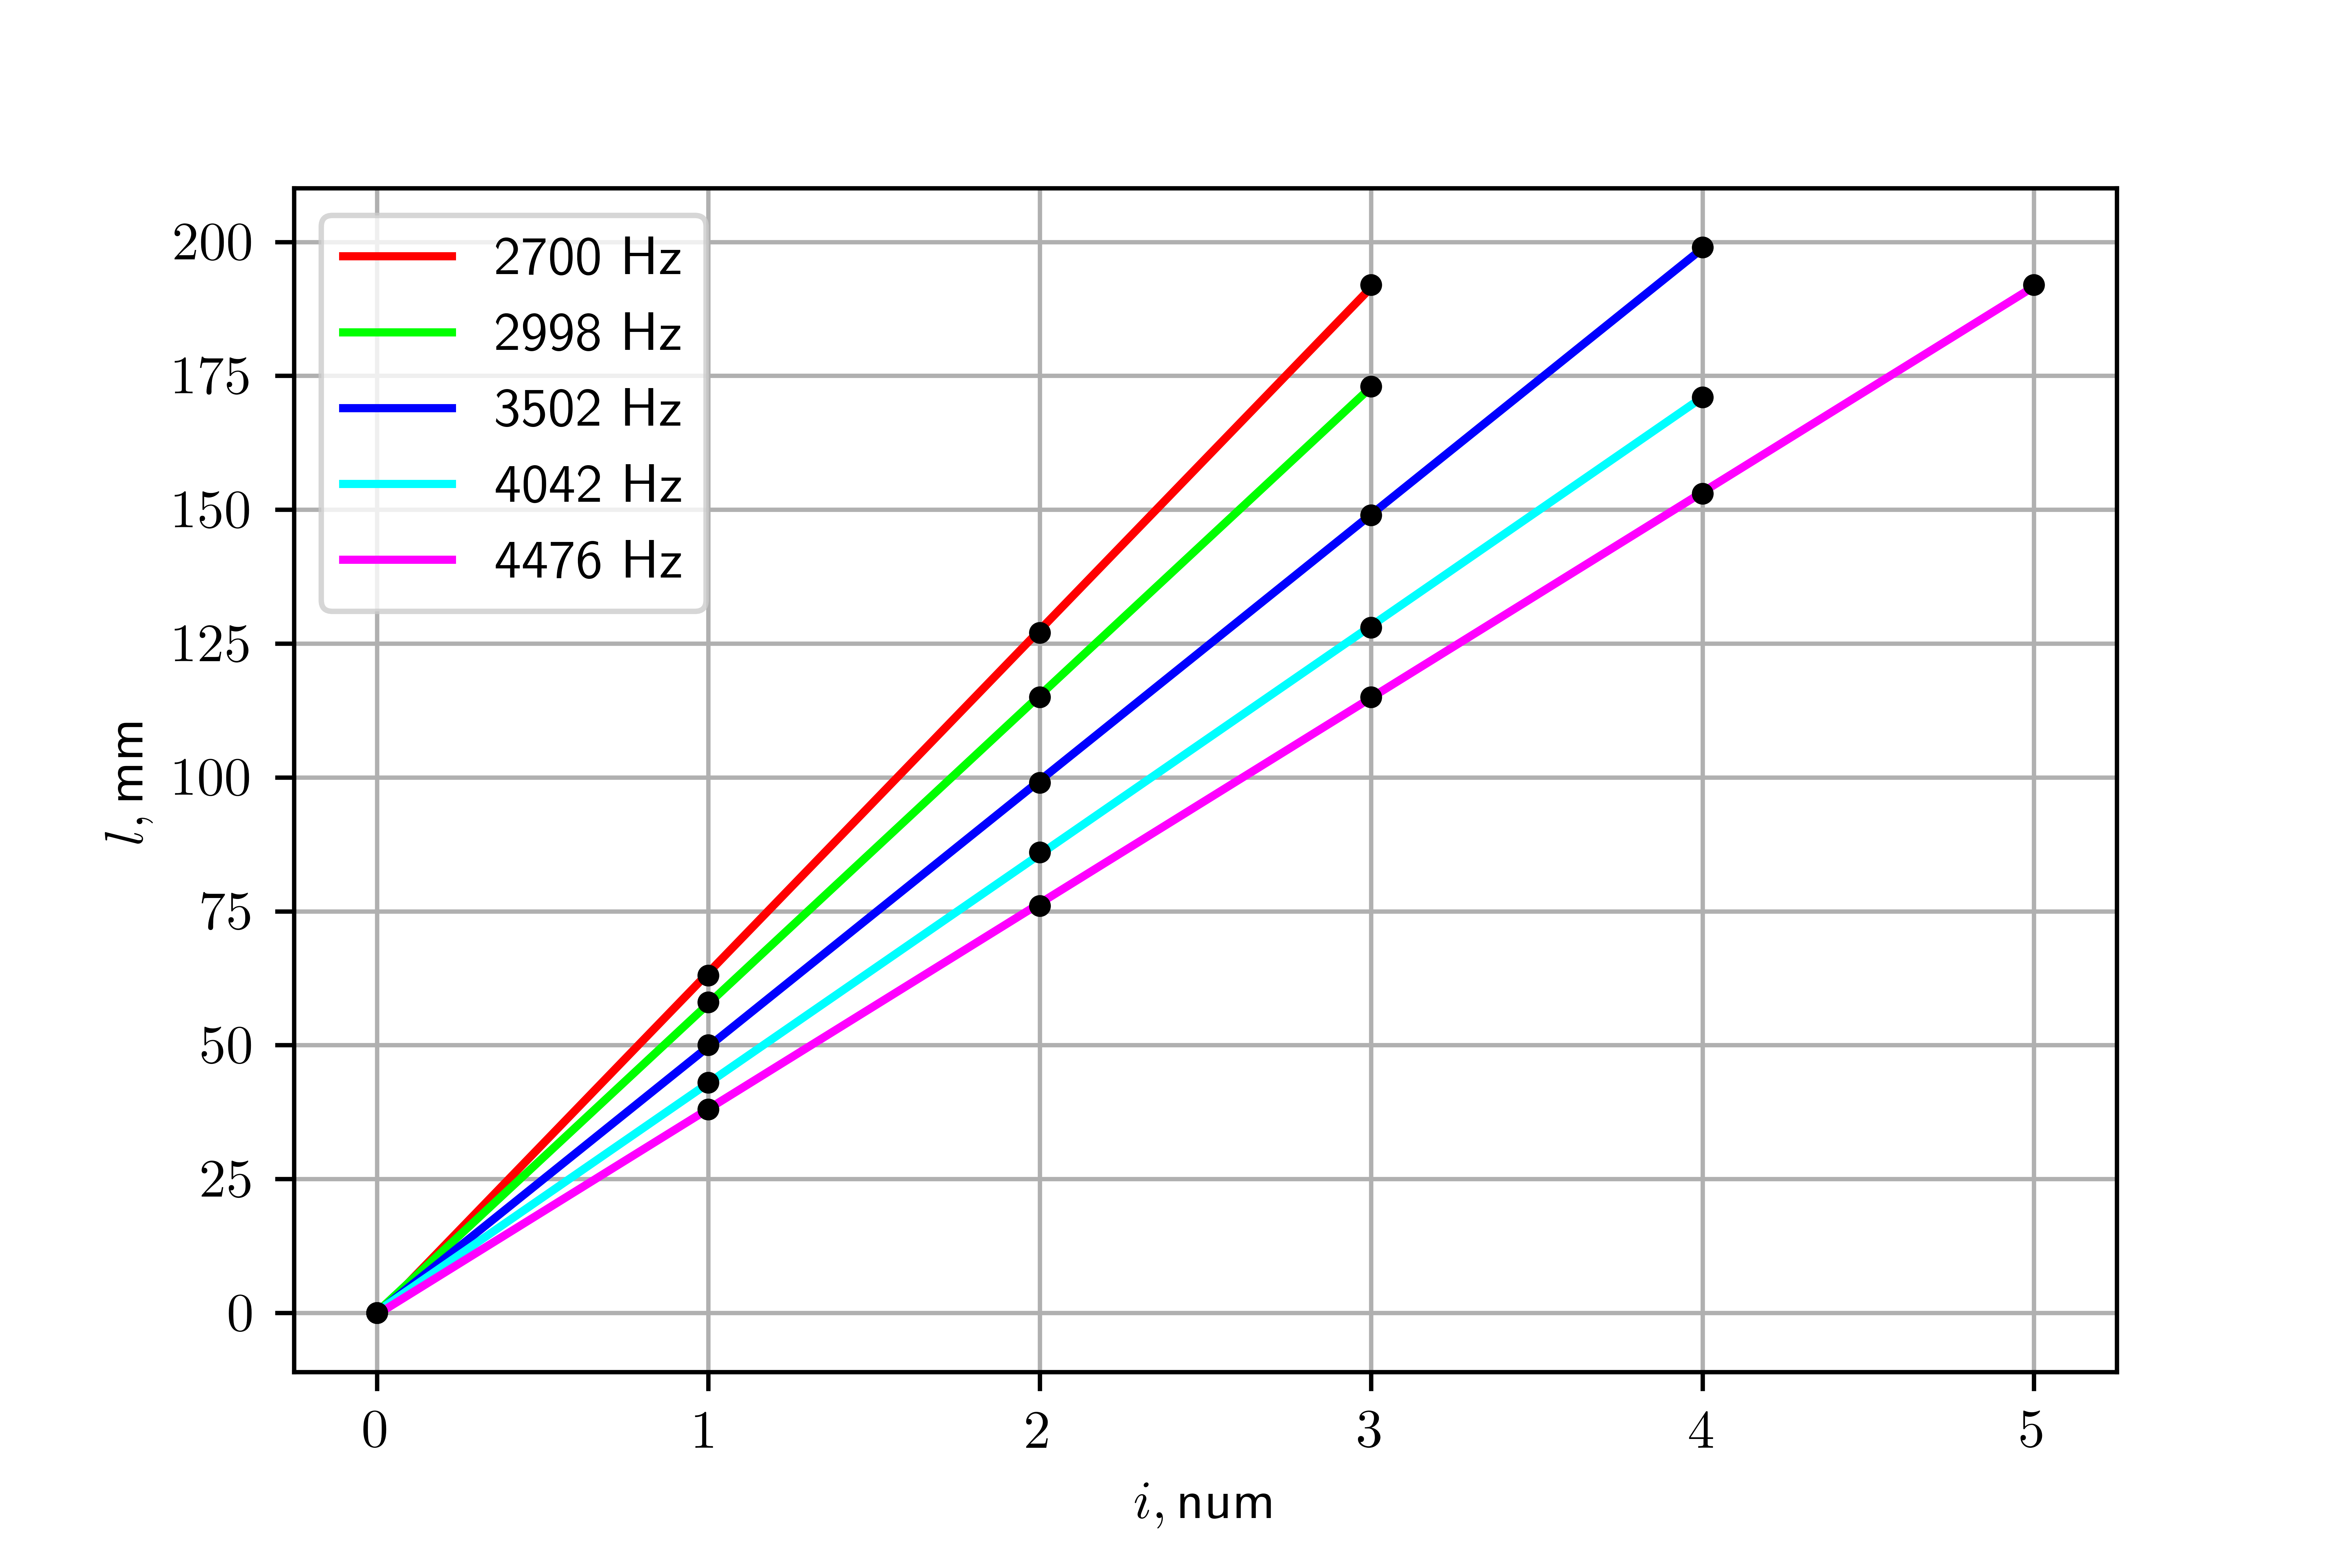
\includegraphics[scale=0.73]{PIC_2.png}
		\\\textbf{Рис. 2:} График зависимостей $l(i)$
	\end{center}

	По построенным графикам определим длины волн и рассчитаем скорости звука.
	
	\begin{center}
		\begin{tabular}{|c|c|c|}
			\hline
			$f$, Гц & $\lambda$, мм & $c$, м/с
			\\\hline
			$2700 \pm 1$ & $128.0 \pm 0.6$ & $345.6 \pm 1.6$
			\\\hline
			$2998 \pm 1$ & $115.2 \pm 0.3$ & $345.4 \pm 0.9$
			\\\hline
			$3502 \pm 1$ & $99.4 \pm 0.2$ & $348.1 \pm 0.7$
			\\\hline
			$4042 \pm 1$ & $85.4 \pm 0.2$ & $345.2 \pm 0.8$
			\\\hline
			$4476 \pm 1$ & $76.8 \pm 0.2$ & $343.8 \pm 0.9$
			\\\hline
		\end{tabular}
		\\\textbf{Табл. 2}: Определение скорости звука
	\end{center}

	Таким образом, усреднением получаем:
	
	$$c = 345.6 \pm 1.0\ \text{м}/\text{с}$$
	
	Вычисляем показатель адиабаты по формуле (1):
	
	$$\gamma_{\text{возд}} = 1.389 \pm 0.008$$
	
	\paragraph{Опыт с переменной длиной трубы для углекислого газа} \hfill
	
	Будем записывать величину вылета трубы для каждого из положений резонанса в таблице для нескольких разных частот звукового генератора на этот раз при подаче углекислого газа в трубу.
	
	\begin{center}
		\begin{tabular}{|c|c|c|c|c|c|}
			\hline
			$f$, Гц & $2204 \pm 1$ &  $2402 \pm 1$ & $2600 \pm 1$ & $2802 \pm 1$ & $3095 \pm 1$
			\\\hline
			$i$, номер & \multicolumn{5}{|c|}{$((l - l_0) \pm 1)$, мм}
			\\\hline
			0 & 0 & 0 & 0 & 0 & 0
			\\\hline
			1 & 62 & 55 & 52 & 49 & 43
			\\\hline
			2 & 122 & 111 & 102 & 97 & 87
			\\\hline
			3 & 183 & 167 & 155 & 145 & 130
			\\\hline
			4 &     &     &     & 193 & 174
			\\\hline
		\end{tabular}
		\\\textbf{Табл. 3:} Второй опыт
	\end{center}

	\newpage

	%Страница 5
	
	\begin{flushleft}
		\footnotesize{Определение $C_p /C_v$ по скорости звука в газе} \hspace{\fill} \footnotesize{5}
		\\[-0.3cm]\noindent\rule{\textwidth}{0.3pt}
	\end{flushleft}

	\begin{center}
		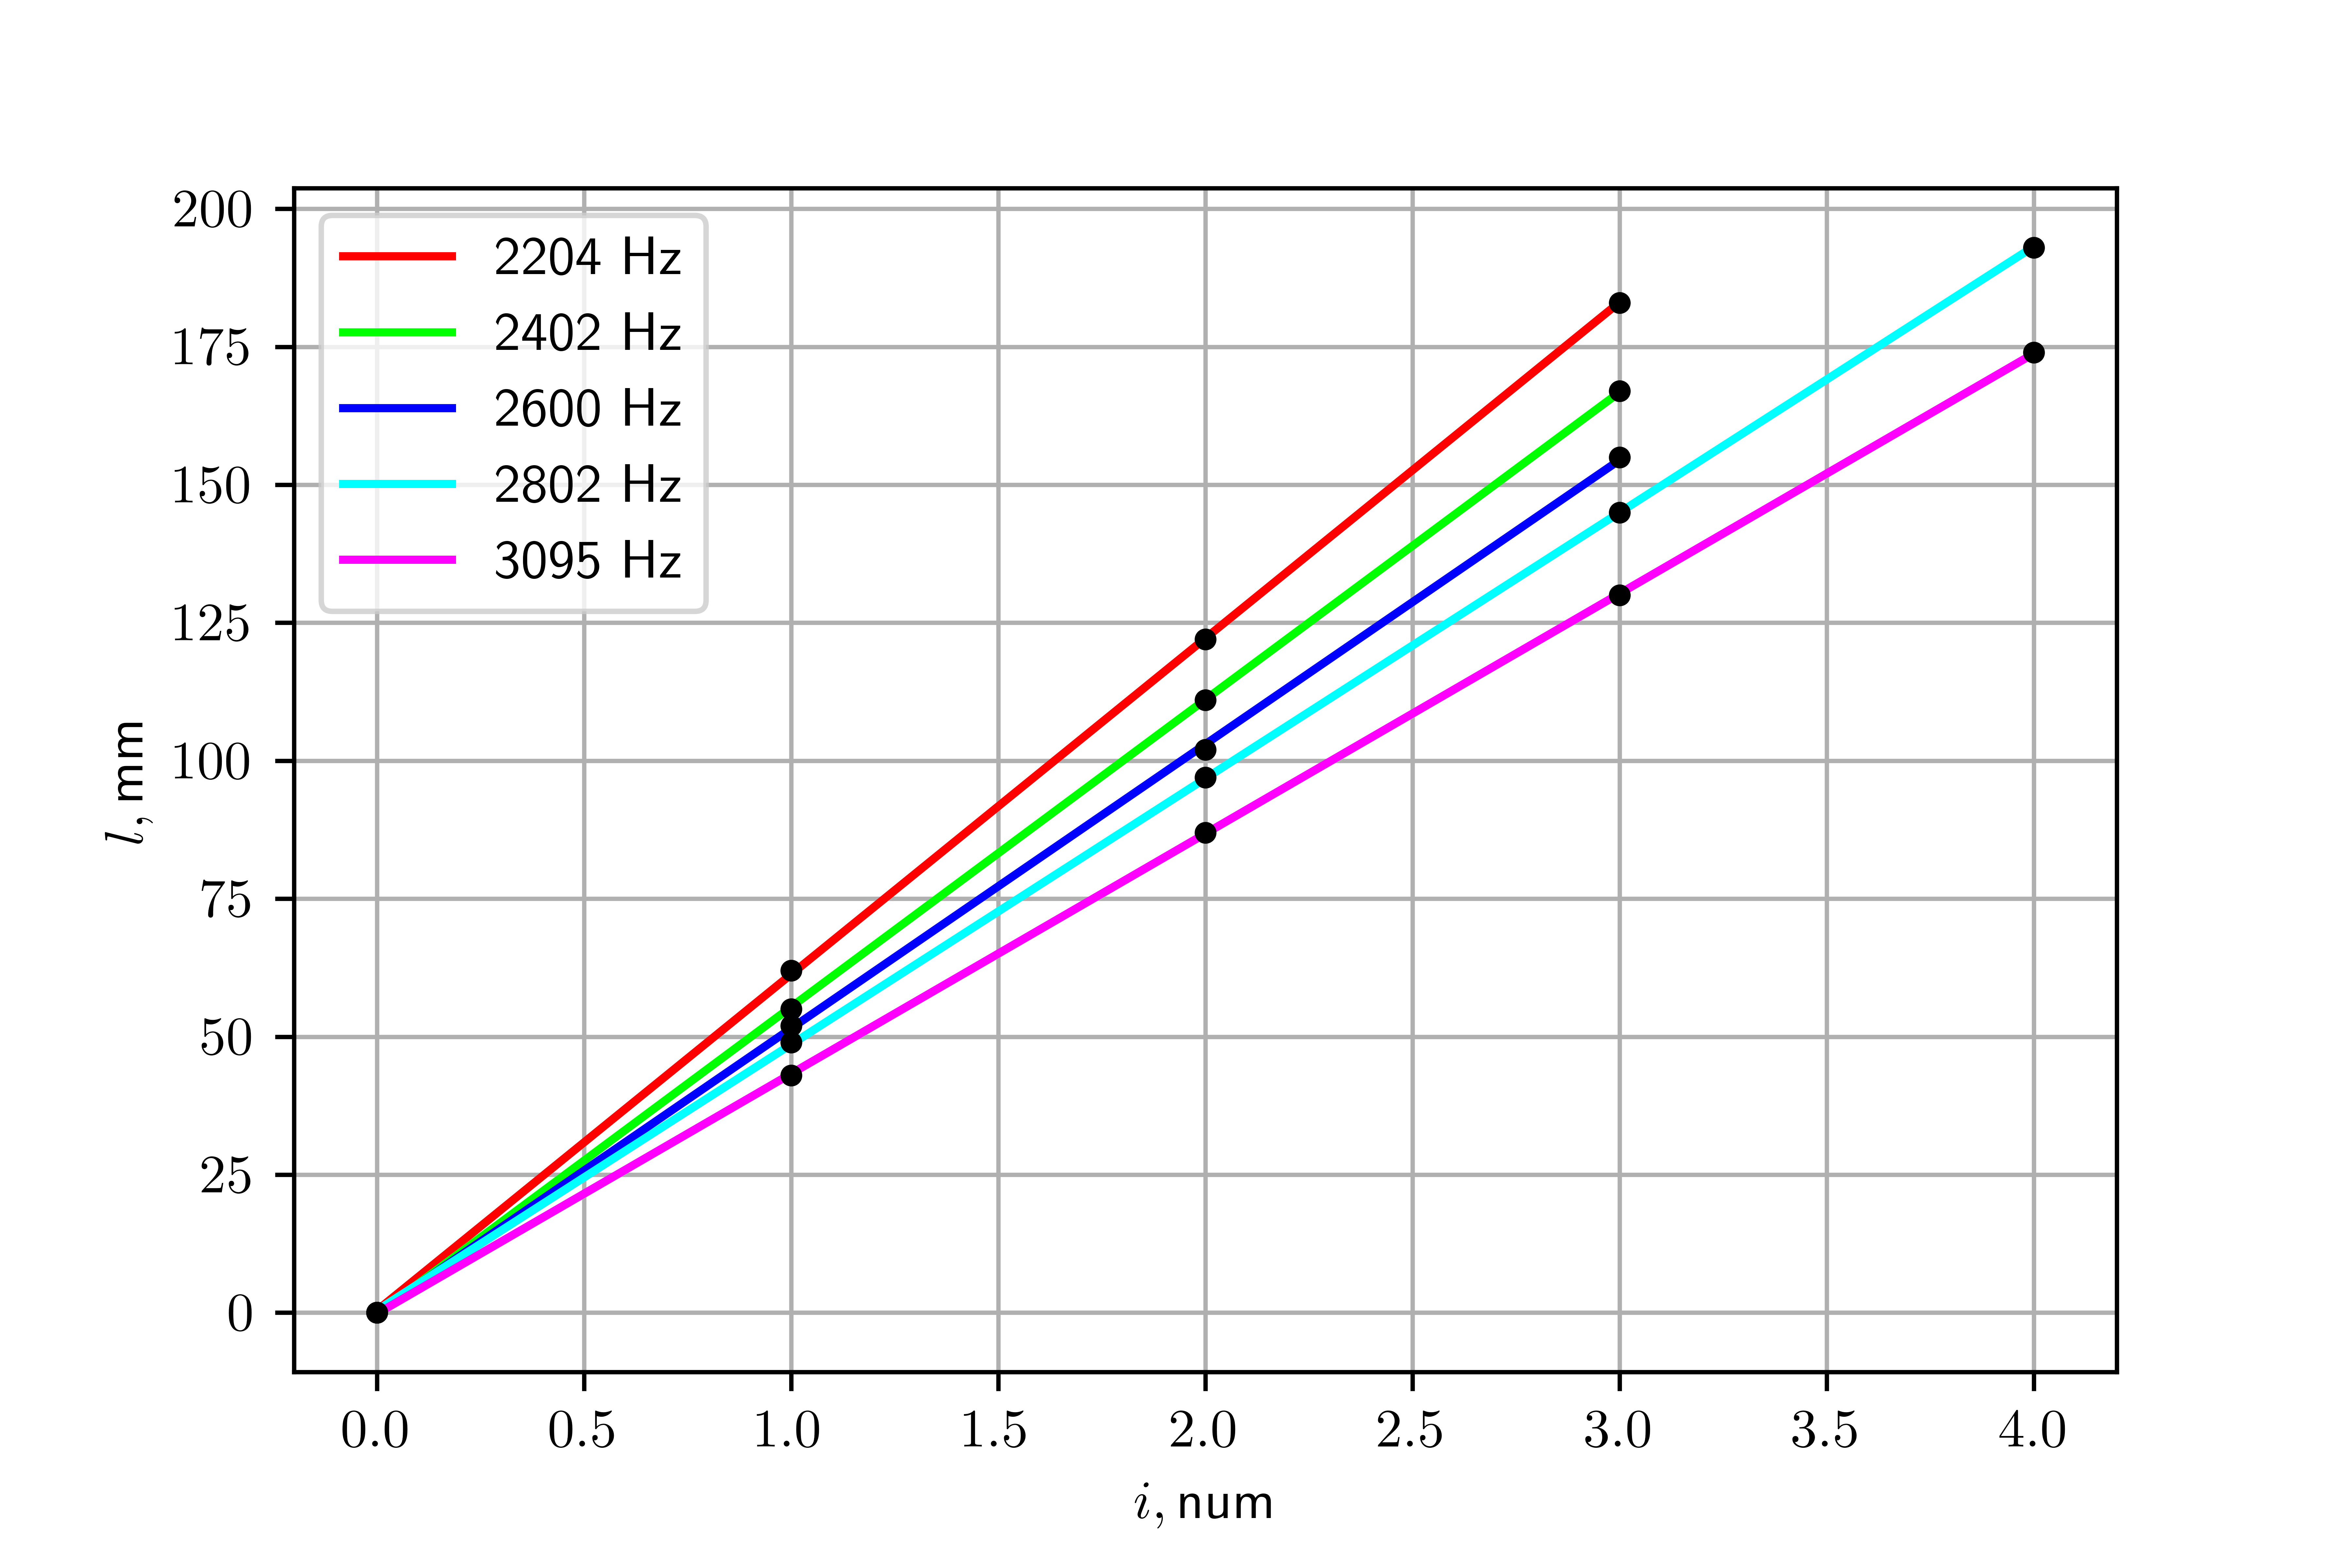
\includegraphics[scale=0.73]{PIC_3.png}
		\\\textbf{Рис. 3:} График зависимостей $l(i)$
	\end{center}
	
	По построенным графикам определим длины волн и рассчитаем скорости звука.
	
	\begin{center}
		\begin{tabular}{|c|c|c|}
			\hline
			$f$, Гц & $\lambda$, мм & $c$, м/с
			\\\hline
			$2204 \pm 1$ & $121.8 \pm 0.5$ & $268.4 \pm 1.1$
			\\\hline
			$2402 \pm 1$ & $111.4 \pm 0.3$ & $267.6 \pm 0.5$
			\\\hline
			$2600 \pm 1$ & $103.0 \pm 0.8$ & $267.8 \pm 2.1$
			\\\hline
			$2802 \pm 1$ & $96.4 \pm 0.2$ & $270.1 \pm 0.6$
			\\\hline
			$3095 \pm 1$ & $87.0 \pm 0.2$ & $269.3 \pm 0.6$
			\\\hline
		\end{tabular}
		\\\textbf{Табл. 4}: Определение скорости звука
	\end{center}
	
	Таким образом, усреднением получаем:
	
	$$c = 268.6 \pm 1.0\ \text{м}/\text{с}$$
	
	Вычисляем показатель адиабаты по формуле (1):
	
	$$\gamma_{\mathrm{CO}_2}} = 1.273 \pm 0.009$$		
		
	\section{Выводы}
	\begin{enumerate}
		\item В результате работы определен показатель адиабаты воздуха:
		
		$$\gamma_{\text{возд}} = 1.389 \pm 0.008$$
		
		Что совпадает с табличным значением $\gamma_{\text{возд}\, 0} = 1.4$ в пределах двух стандартных отклонений.
		
		\item Получено значение показателя адиабаты и для углекислого газа:
		
		$$\gamma_{\mathrm{CO}_2}} = 1.273 \pm 0.009$$		
		
		Что также совпадает с табличным значением $\gamma_{\mathrm{CO}_2}\б 0} = 1.3$ в пределах двух стандартных отклонений.
	\end{enumerate}
	
	
	Таким образом, в целом, работа проведена успешно. Худшее совпадение для углекислого газа можно объяснить наличием примесей (в основном, азот и кислород) в атмосфере трубы, так как труба была не до конца герметична.
		
\end{document}